\documentclass[a4paper]{article}

\usepackage[portuguese]{babel}
\usepackage[utf8]{inputenc}
\usepackage{graphicx,hyperref}
\usepackage{float}
\usepackage{listings}
\usepackage{proof,tikz}
\usepackage{algorithm2e}
\usepackage{amssymb,amsthm,stmaryrd}


\usepackage[edges]{forest}
\usetikzlibrary{automata, positioning, arrows}


\newtheorem{Lemma}{Lema}
\newtheorem{Theorem}{Teorema}
\theoremstyle{definition}
\newtheorem{Example}{Exemplo}
\newtheorem{Definition}{Definição}


\usepackage{fancyhdr}
  \pagestyle{fancy}
  \fancyhf{}
  \lhead{Teoria da Computação}
  \rhead{Aula 20}
  \lfoot{Prof. Rodrigo Ribeiro}
  \rfoot{\thepage}
  \renewcommand{\footrulewidth}{0.4pt}
  \pagestyle{fancy}

\tikzset{
        ->,  % makes the edges directed
        >=stealth', % makes the arrow heads bold
        node distance=3cm,
        every state/.style={thick, fill=gray!10},
        initial text=$\,$
        }
  

\begin{document}

\title{Aula 20 - Gramáticas, Máquinas de Turing e\\ Propriedades de Fechamento
  de Linguagens Recursivas e Recursivamente Enumeráveis}
  \author{Rodrigo Ribeiro}

  \maketitle

  

  \pagestyle{fancy}


  \section*{Objetivos}

  \begin{itemize}
     \item Apresentar a equivalência de máquinas de Turing e gramáticas
       irrestritas.
     \item Apresentar os conceitos de autômato linearmente limitado,
       gramática sensível ao contexto e linguagem sensível ao contexto.
     \item Apresentar a hierarquia de Chomsky.
     \item Apresentar as propriedades de fechamento para as classes de
           linguagens recursivas e recursivamente enumeráveis.
  \end{itemize}

  \section{Equivalência entre Gramáticas e MTs}


  \begin{Definition}[Gramática irrestrita]
    Seja $G = (V,\Sigma, R, P)$ uma gramática. Dizemos que $G$ é irrestrita
    se toda regra de $R$ possui a forma $x \to y$, em que $x \in (V\cup
    \Sigma)^+$ e $y \in (V\cup \Sigma)^*$.
  \end{Definition}

  \begin{Theorem}
    A linguagem gerada por uma gramática irrestrita é uma linguagem
    recursivamente enumerável.
  \end{Theorem}
  \begin{proof}
    Seja $G = (V,\Sigma,R,P)$ uma gramática irrestrita. Para mostrar que $G$
    produz uma linguagem recursivamente enumerável, mostraremos (informalmente)
    como construir
    uma MT $M$ de duas fitas não determinística tal que $L(G) = L(M)$.
    A fita $1$ de $M$ armazenará a palavra de entrada, que não será modificada,
    e a fita $2$ uma etapa da derivação de $w$ em $G$. O seguinte algoritmo
    descreve os passos a serem realizados pela MT em alto nível.
    
    \begin{algorithm}[H]
      Escreva $P$ (variável de partida) na fita 2 \;
      \While {true}{
        Selecione uma posição $p$ na palavra contida na fita 2 (Não determinismo)\; 
        Selecione uma regra $u \to v \in R$ (Não determinismo)\;
        \eIf{se $u$ ocorre a partir da posição $p$ da fita 2}{
          Substitua $u$ por $v$ na fita 2 \;
          \If{Se a palavra na fita $2$ for igual a da fita 1}{Aceite \;}
        }{
          Rejeite \;
        }
      }  
    \end{algorithm}    
  \end{proof}

  \begin{Theorem}
    Uma linguagem recursivamente enumerável pode ser gerada por uma gramática
    irrestrita.
  \end{Theorem}
  \begin{proof}
    Seja $L$ uma linguagem recursivamente enumerável e uma MT $M = (E,\Sigma,\Gamma,
    \langle, \sqcup, \delta,i,F)$ tal que $L(M) = L$. Mostraremos que
    existe uma gramática irrestrita $G = (V,\Sigma,R,P)$ que gera $L$.
    Informalmente, $G$ possuirá regras para:
    \begin{enumerate}
      \item Gerar formas sentenciais do tipo $w\langle i w \rangle$, em que $w
        \in \Sigma^*$ e os símbolos $i, \langle, \rangle$ são variáveis em $G$.
      \item Simular a execução de $M$ sobre a configuração instantânea $\langle
        i w\rangle$, deixando o prefixo $w$ inalterado.
      \item Apagar a configuração instantânea quando ela for da forma 
        $\langle x e a y \rangle$, em que $e \in F$ e $\delta(e,a) = \bot$.
    \end{enumerate}
    A primeira etapa é construir regras para produzir $w\langle i w\rangle$. 
    Seja $\Sigma = \{a_1,...,a_n\}$. Para cada $a_i \in \Sigma$ criaremos uma
    variável $A_i$ em $G$ e uma variável $B$, diferente de todo $A_i$. Criamos
    então as seguintes regras.
    \[
      \begin{array}{lcl}
        P & \to & B \rangle \\
        B & \to & a_kBA_k, 1 \leq k \leq n \\
        B & \to & \langle i\\
        A_k & \to & a_k\rangle, 1 \leq k \leq n \\
        A_ja_k & \to & a_kA_j, 1 \leq j, k \leq n\\ 
      \end{array}
    \]
    A segunda parte das regras simula a execução de $M$ sobre $\langle iw
    \rangle$.
    \begin{itemize}
       \item Para cada transição da forma $\delta(e,a) = [e',b,D]$:
         \[
           \begin{array}{lcl}
             ea & \to & be' \\
             e\rangle & \to & be'\rangle, \textit{ se } a = \sqcup\\
           \end{array}
         \]
       \item Para cada transição da forma $\delta(e,a) = [e',b,E]$:
         \[
           \begin{array}{lcl}
             cea & \to & e'cb, \textit{ para cada }c \in \Gamma\\
             ce\rangle & \to & e'cb\rangle, \textit{ para cada } c \in \Gamma, a = \sqcup
           \end{array}
         \]
       \end{itemize}
       Finalmente, resta regras para apagar a configuração instantânea quando
       esta for da forma $\langle x e a y \rangle$, com $e \in F$ e $\delta(e,a)
       = \bot$. Para isso, introduz-se uma variável nova \#:
       \begin{itemize}
          \item Para cada par $(e,a)$ tal que $e\in F$ e $\delta(e,a) = \bot$:
            \[
              \begin{array}{lcl}
                ea & \to & a\# \\
                e\rangle & \to & \#\rangle, \textit{se }a = \sqcup\\
                \#c & \to & \#, c \in \Gamma - \{\langle\}\\
                c\# & \to & \#, c \in \Gamma - \{\langle\}\\
                \langle \# \rangle & \to & \lambda\\
              \end{array}
            \]
       \end{itemize}
  \end{proof}

  Apresentamos um exemplo para ilustrar essa construção de gramática em termos
  de uma MT.

  \begin{Example}
    Vamos utilizar a construção do teorema anterior para construir a gramática
    irrestrita correspondente a seguinte MT:
    \begin{figure}[H]
      \begin{tikzpicture}[node distance=3cm]
        \node[state, initial, accepting](s0){$e$};
        \node[state, right of=s0](s1){$e'$};
        
        \draw (s0)edge[loop above]node{$1/1\,D$}(s0)
              (s0)edge[above, bend left] node{$0/0\,D$}(s1)
              (s1)edge[loop above]node{$1/1\,D$}(s1)
              (s1)edge[below, bend left] node{$0/0\,D$}(s0);
      \end{tikzpicture}
      \centering
    \end{figure}
    Vamos considerar a palavra $w = 00$. Logo, temos as seguintes regras para
    construir a configuração inicial.
    \[
      \begin{array}{lcl}
        P & \to & B \rangle \\
        B & \to & 0 B Z \,|\, 1 B U \,|\, \langle e \\
        Z \rangle & \to & 0 \rangle \\
        U \rangle & \to & 1 \rangle \\
      \end{array}
    \]
    Agora, vamos apresentar as regras para cada uma das transições.
    \begin{itemize}
       \item Transição $\delta(e,0) = [e',0, D]$.
         \[
           \begin{array}{lcl}
             e0 & \to & 0e' \\
           \end{array}
         \]
       \item Transição $\delta(e,1) = [e,1,D]$.
         \[
           \begin{array}{lcl}
             e1 & \to & 1e\\
           \end{array}
         \]
       \item Transição $\delta(e',1) = [e',1,D]$.
         \[
           \begin{array}{lcl}
             e'1 & \to & 1e'\\
           \end{array}           
         \]
       \item Transição $\delta(e',0) = [e,0, D]$.
         \[
           \begin{array}{lcl}
             e'0 & \to & 0e \\
           \end{array}
         \]    
     \end{itemize}
     Finalmente, incluimos regras para apagar a configuração $\langle x e a y
     \rangle$.
     \begin{itemize}
        \item Para $\delta(e,\sqcup) = \bot$, temos:
          \[
            \begin{array}{lcl}
              e\sqcup & \to & \langle\# \\
              e\rangle & \to & \#\rangle\\
              \#0     & \to & \# \\
              \#1     & \to & \# \\
              \langle \# \rangle & \to & \lambda \\
            \end{array}
          \]
        \end{itemize}
       Desta forma, temos que o conjunto total de regras da gramática é dado
       por:
       \[
         \begin{array}{lcl}
        P & \to & B \rangle \\
        B & \to & 0 B Z \,|\, 1 B U \,|\, \langle e \\
        Z \rangle & \to & 0 \rangle \\
        U \rangle & \to & 1 \rangle \\
             e0 & \to & 0e' \\
           e1 & \to & 1e\\
           e'1 & \to & 1e'\\
           e'0 & \to & 0e \\
              e\sqcup & \to & \langle\# \\
              e\rangle & \to & \#\rangle\\
              \#0     & \to & \# \\
              \#1     & \to & \# \\
              \langle \# \rangle & \to & \lambda \\           
         \end{array}
       \]       
     \end{Example}

     \section{Autômatos Linearmente Limitados}

     \begin{Definition}[Autômato linearmente limitado]
       Um autômato linearmente limitado (ALL) é uma máquina de Turing não
       determinística, $M=(E,\Sigma,\Gamma,\langle,\rangle,\delta,i,F)$,
       em que:
       \begin{itemize}
         \item $\rangle$ é um símbolo especial que não pode ser escrito na fita;
         \item A configuração inicial é $[i,\langle w \rangle]$ ; e
         \item Se $\delta(e,\rangle)$ é definida, então $\delta(e,\rangle) =
           [e',\rangle,E]$ para algum $e' \in E$.
       \end{itemize}
     \end{Definition}

     \begin{Example}
       A linguagem $\{a^nb^nc^n\,|\,n \geq 0\}$ é reconhecida pelo seguinte ALL: 
       \begin{figure}[H]
         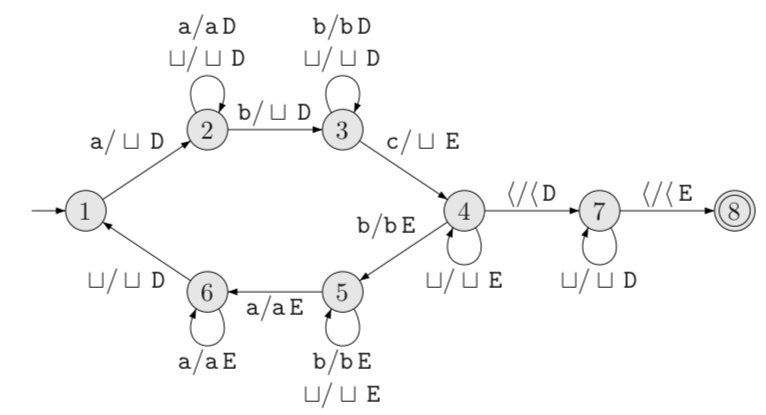
\includegraphics[scale=.3]{all.png}
         \centering
       \end{figure}
     \end{Example}

     \begin{Definition}[Gramática sensível ao contexto]
       Uma gramática $G = (V,\Sigma,R,P)$ é dita ser sensível ao contexto (GSC)
       se toda regra $x \to y \in R$ é tal que $x,y\in (V\cup\Sigma)^*$ e $|x|
       \leq |y|$.
     \end{Definition}

     \begin{Example}
       A seguir apresentamos uma GSC que gera a linguagem $\{a^nb^nc^n\,|\,n
       \geq 0\}$.
       \[
         \begin{array}{lcl}
           P & \to & aPBc \,|\,abc\\
           cB & \to & Bc \\
           bB & \to & bb\\
         \end{array}
       \]
     \end{Example}

     \begin{Definition}[Linguagem sensível ao contexto]
       Uma linguagem é dita ser sensível ao contexto (LSC) se existe uma
       gramática sensível ao contexto que a gere.
     \end{Definition}

     Desta forma, temos que se $\lambda \in L$, então $L$ não é uma $LSC$, visto
     que $GSC$ não podem gerar $\lambda$.

     \section{A hierarquia de Chomsky}

     Com a apresentação dos ALLs completamos a caracterização de linguagens
     formais, seus reconhecedores e suas respectivas gramáticas. A tabela
     seguinte resume esses resultados.
     
     \begin{table}[H]
       \begin{tabular}{|l|l|l|}
         \hline
         Classe & Reconhecedor & Gramática \\ 
         \hline 
         Ling. Reg. & AFD & Gram. Regular \\ 
         Ling. Livre Cont. & APN & Gram. Livre cont. \\
         Ling. Sens. Cont. & ALL & Gram. Sens. cont.\\
         Ling. Rec. & MTs & Gram. irrestritas \\
         Ling. Rec. En. & MTs & Gram. irrestritas\\ \hline
       \end{tabular}
       \centering
     \end{table}

     Note que é possível construir um $AP$ que simule um $AFD$ qualquer. Além
     disso, existem linguagens aceitas por $APs$ que não podem ser reconhecidas 
     por AFs quaisquer. Logo, podemos concluir que a classe das linguagens
     regulares é um subconjunto próprio da classe das linguagens livres de
     contexto, i.e., $LRs \subset LLCs$.

     De maneira similar, pode-se mostrar que existem $LSCs$ que não são aceitas
     por nenhum $AP$ e que, a menos de linguagens $L$ tais que $\lambda \in L$,
     ALLs podem simular quaisquer APs. Logo, as linguagens livres de contexto
     são um subconjunto próprio de linguagens sensíveis ao contexto.

     As linguagens sensíveis ao contexto podem ser reconhecidas por MTs que
     sempre param. Logo, podemos dizer que as linguagens sensíveis ao contexto
     são um subconjunto próprio de linguagens recursivas. Como linguagens
     recursivas são as que possuem MTs que as aceitam e param para todas as
     possíveis entradas e linguagens recursivamente enumeráveis são as que são
     possuem MTs que as aceitam, temos que a classe das linguagens recursivas é
     um subconjunto próprio das linguagens recursivamente enumeráveis.

     Do apresentado acima, podemos concluir a seguinte hierarquia de linguagens:

     \[
       LRs \subset LLCs \subset LSCs \subset LRecs \subset LREs \subset \mathcal{P}(\Sigma^*)
     \]

     Note que a hierarquia acima, além de mostrar a relação de subconjunto entre
     diferentes classes de linguagens, também mostra o crescente poder
     computacional de reconhecedores e de suas gramáticas. Essa hierarquia que
     define o poder de máquinas, gramáticas e suas respectivas classes de
     linguagens é chamada de hierarquia de Chomsky. A figura abaixo ilustra esse
     relacionamento entre as diferentes classes de linguagens formais.

       \begin{figure}[H]
         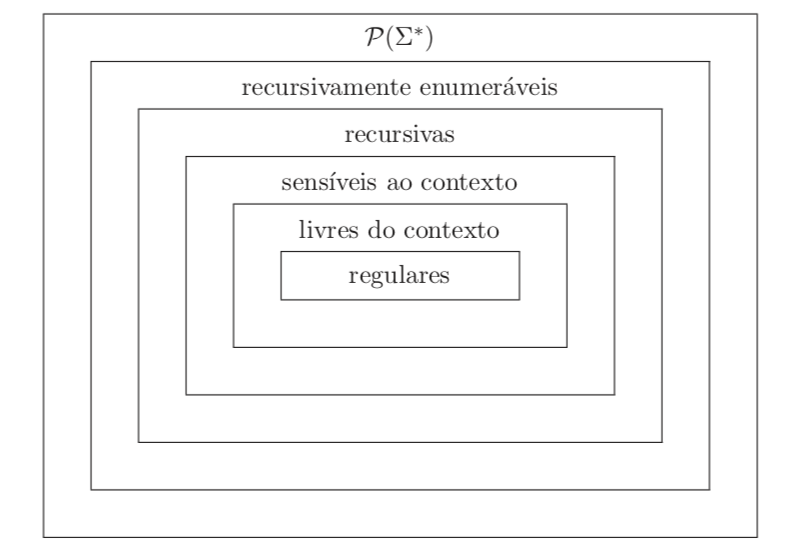
\includegraphics[scale=.3]{chomsky.png}
         \centering
       \end{figure}

       \section{Propriedades de Fechamento de LREs e das Linguagens Recursivas}

       \begin{Theorem}
         A classe das linguagens recursivas é fechada sobre união, interseção e
         complementação
       \end{Theorem}
       \begin{proof}
         Sejam $M_1=(E_1,\Sigma, \Gamma, \langle, \sqcup, \delta_1, i_1,F_1)$ e
         $M_2=(E_2,\Sigma, \Gamma, \langle, \sqcup, \delta_2, i_2,F_2)$
         duas MTs que aceitam linguagens recursivas. Para mostrar o fechamento
         com respeito a interseção e união, utilizaremos a mesma técnica
         utilizada para AFs: simular a execução em paralelo. Para isso, vamos
         construir uma MT $M=(E,\Sigma, \Gamma, \langle, \sqcup,\delta, i,F)$,
         em que:
         \begin{itemize}
            \item $E = (E_1 \times E_2) \cup\{i,j\}$
         \end{itemize}
         Para facilitar, $M$ será uma MT de duas fitas em que a primeira
         simulará a execução de $M_1$ e a segunda a execução de $M_2$. Para
         isso, primeiramente copiamos a palavra de entrada da fita 1 para a fita
         2 usando as seguintes transições:
         \begin{itemize}
           \item $\delta(i,a,\sqcup) = [i,[a,D],[a,D]]$ para todo $a\in \Sigma$;
           \item $\delta(i,\sqcup,\sqcup) = [j,[\sqcup,E],[\sqcup,E]]$
           \item $\delta(j,a,a) = [j,[a,E],[a,E]]$, para todo $a\in\Sigma$;
           \item $\delta(j,\langle, \langle) = [[i_1,i_2],[\langle, D],[\langle,D]]$.
         \end{itemize}
         Logo após a cópia da palavra de entrada, a MT começa a operar no estado
         $[i_1,i_2]$. O restante de $\delta$ é construído a partir de $\delta_1$
         e $\delta_2$ da seguinte maneira:
         \begin{itemize}
           \item Se $\delta_1(e_1,a_1) = [e'_1,b_1,d_1]$ e $\delta_1(e_2,a_2) =
             [e'_2,b_2,d_2]$ então, $\delta([e_1,e_2],a_1,a_2) =
             [[e'_1,e'_2],[b_1,d_1],[b_2,d_2]]$; 
           \item Se $\delta_1(e_1,a_1) = \delta_2(e_2,a_2) = \bot$ então 
             $\delta([e_1,e_2],a_1,a_2) = \bot$.
           \item Se $\delta_1(e_1,a_1) = [e'_1,b_1,d_1]$ e $\delta_2(e_2,a_2) =
             \bot$, então $\delta([e_1,e_2],a_1,a_2) =
             [[e'_1,e_2],[b_1,d_1],[a_2,I]]$.
           \item Se $\delta_1(e_1,a_1) = \bot$ e $\delta_2(e_2,a_2) =
             [e'_2,b_2,d_2]$, então $\delta([e_1,e_2],a_1,a_2) =
             [[e_1,e'_2],[a_1,I],[b_2,d_2]]$.           
         \end{itemize}
         Para completar a construção para união basta fazer $F = (F_1 \times
         E_2) \cup (E_1\times F_2)$ e para interseção $F = F_1 \times F_2$.

         Finalmente, uma $MT$ que aceita $\overline{L(M_1)}$ é
         $M=(E_1,\Sigma, \Gamma, \langle, \sqcup, \delta_1, i_1,E_1 - F_1)$.
       \end{proof}

       \begin{Theorem}
         A classe das linguagens recursivamente enumeráveis é fechada sobre
         união e interseção.
       \end{Theorem}
       \begin{proof}
         Construção análoga a de linguagens recursivas.
       \end{proof}

       Observe que as linguagens recursivamente enumeráveis não são fechadas
       sobre a complementação, visto que essa classe possui linguagens para as
       quais não existem MTs que param para toda entrada. Veremos um exemplo de
       tal linguagens em aulas posteriores.

       O seguinte teorema mostra uma importante propriedade de linguagens
       recursivas.

       \begin{Theorem}
         Se $L$ e $\overline{L}$ são linguagens recursivamente enumeráveis,
         então $L$ é uma linguagem recursiva.
       \end{Theorem}
       \begin{proof}
         Consequência do fechamento sobre união.
       \end{proof}
       
  \section{Exercícios}

  \begin{enumerate}
     \item Considere a seguinte linguagem $00(0 + 1)^*$. Apresente uma MT padrão
       que reconheça essa linguagem e construa a gramática irrestrita
       equivalente a sua MT.
  \end{enumerate}
\end{document}
